\chapter{The Standard Model of Particle Physics}
\label{chap:sm}

The discovery of the Higgs (H) boson in 2012 was a monumental achievement solidifying the SM as it found the final fundamental particle within the theory.\cite{201230}  A diagram of the current knowledge of fundamental particles of the SM is seen in Figure \ref{fig:sm}.

\begin{figure}[htbp]
\centering
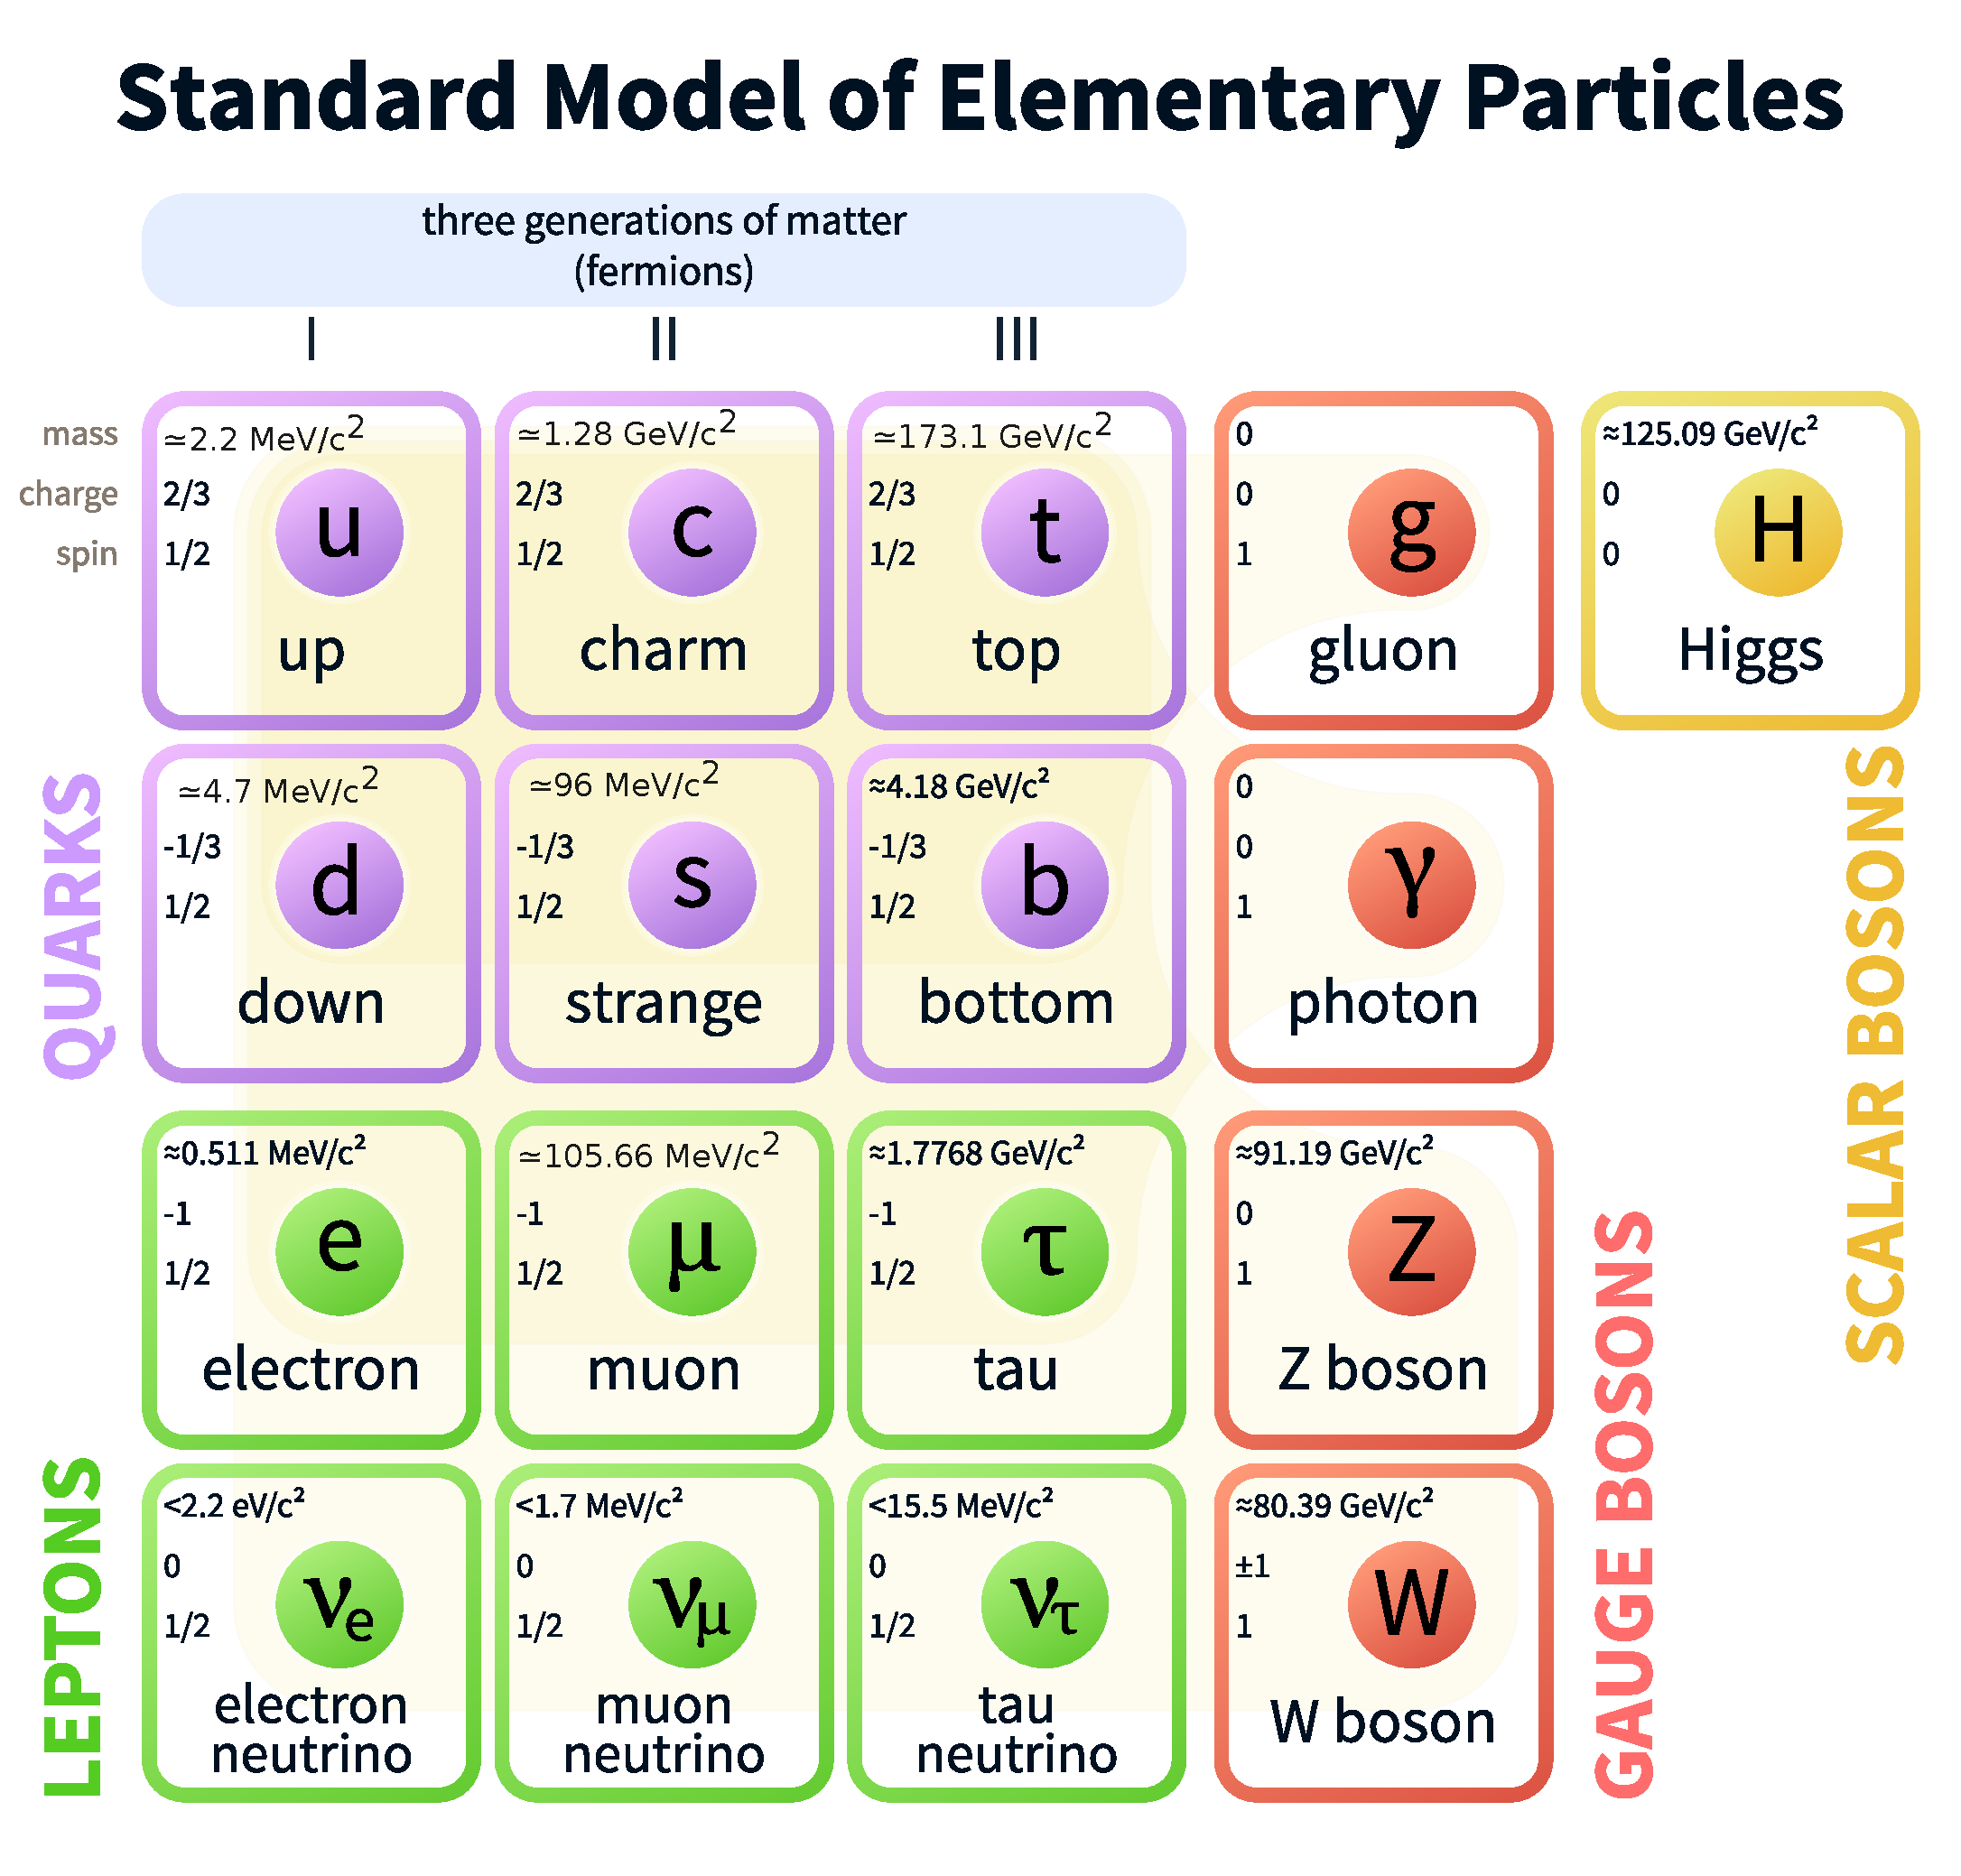
\includegraphics[width=0.75\textwidth]{figs/StandardModelofElementaryParticles.pdf}
\caption{The particles of the Standard Model.}
\label{fig:sm}
\end{figure}

\subsection{Electroweak Theory}
\subsection{Quantum Chromodynamics}
